%=========================================================================
% Member 4 sections: 3.1, 3.3, 3.6, 3.7, 5.2
% This file is generated by code/_sync_sections.py -- edit the
% sections/member4_<n>.tex files instead, then re-run the sync script.
% Requires in preamble (add alongside existing \usepackage lines):
%   \usepackage{booktabs}   % also fixes the current \toprule compile error
%   \usepackage{url}        % \url in the bibliography (also missing upstream)
%=========================================================================

% Member 4 - Section 3.1 Overall Framework
\subsection{Overall Framework}
\label{sec:overall_framework}

Fig.~\ref{fig:framework} summarizes the pipeline. All three experimental groups share one architecture, one set of data splits, and one evaluation protocol, and differ in exactly one factor: the set of images used for training.

\begin{figure}[t]
\centering
% Overall framework diagram. Source: figures/framework.mmd (Mermaid).
% Render with:  npx -y @mermaid-js/mermaid-cli -i figures/framework.mmd -o figures/framework.pdf -b white -s 2
% If the PDF is absent, fall back to the PNG, and finally to a placeholder.
\IfFileExists{figures/framework.pdf}{%
  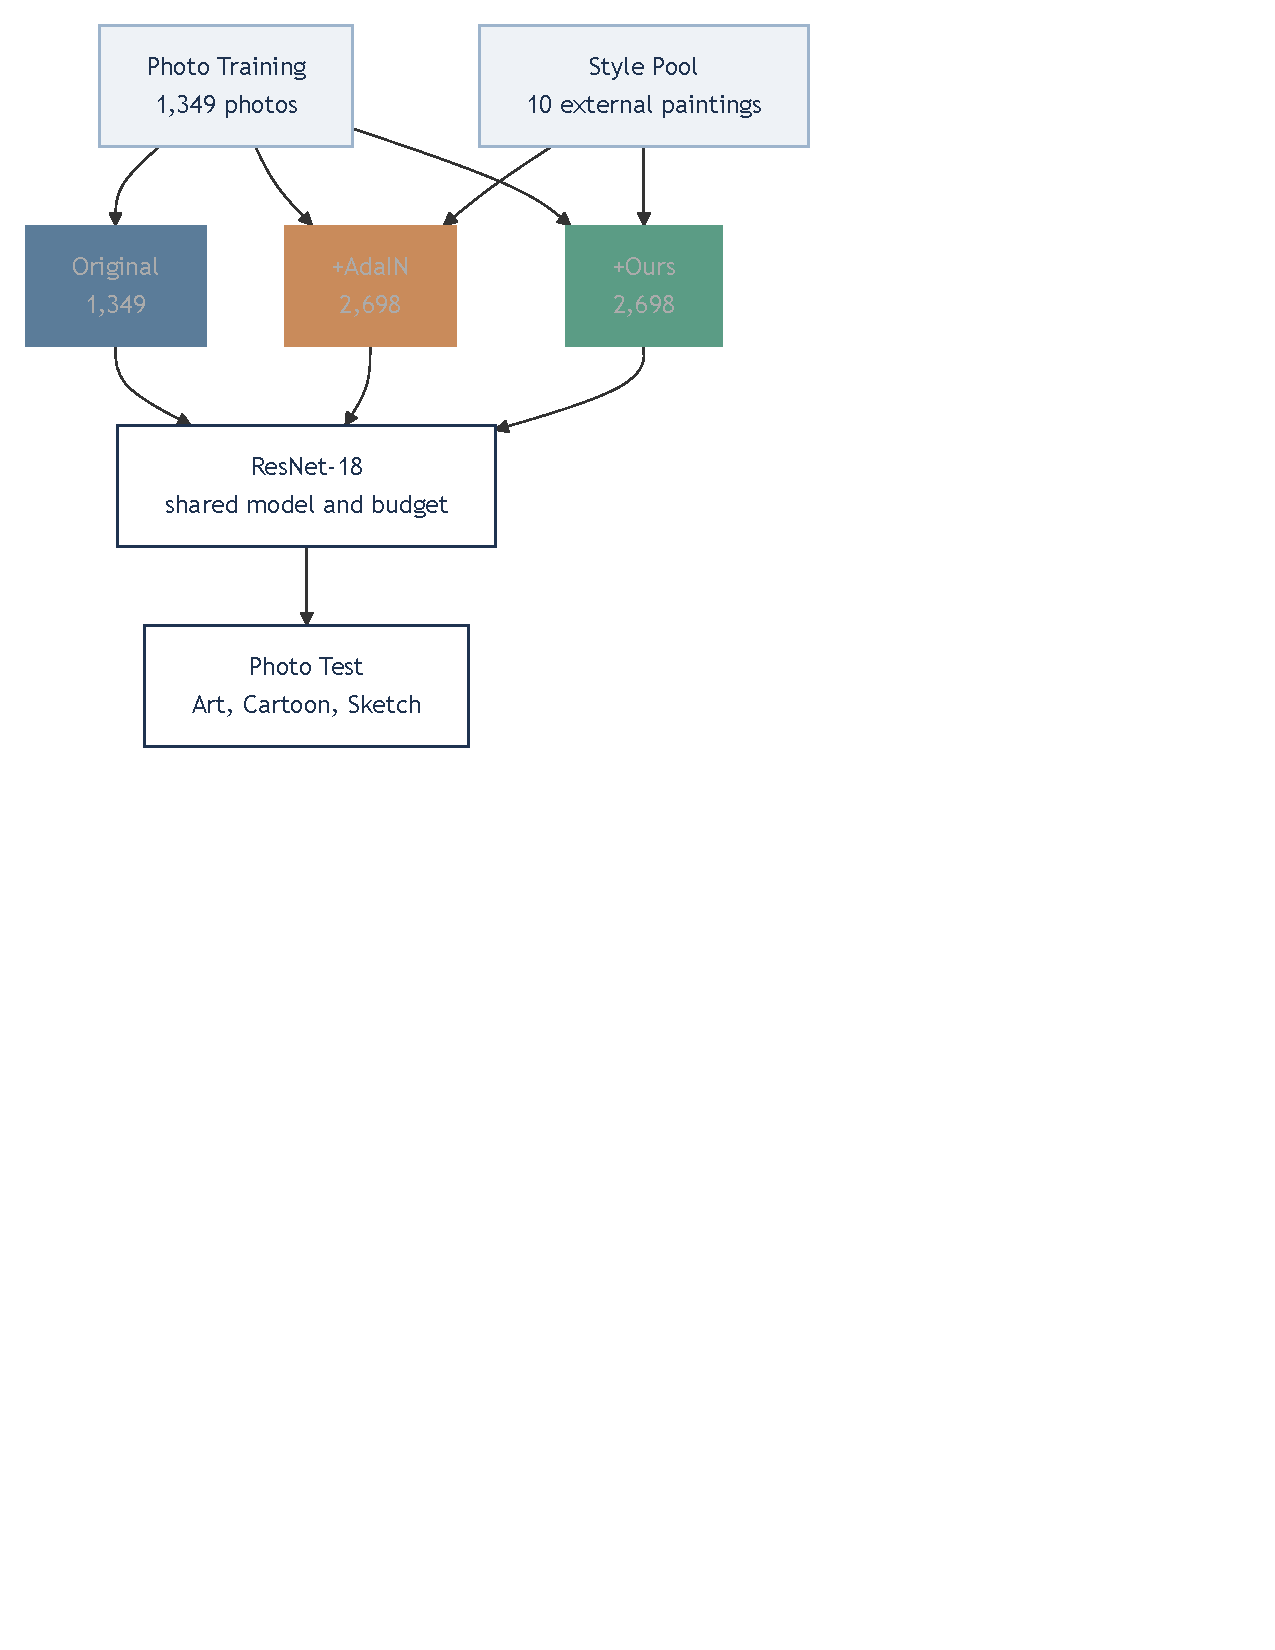
\includegraphics[width=\columnwidth]{figures/framework.pdf}%
}{%
  \IfFileExists{figures/framework.png}{%
    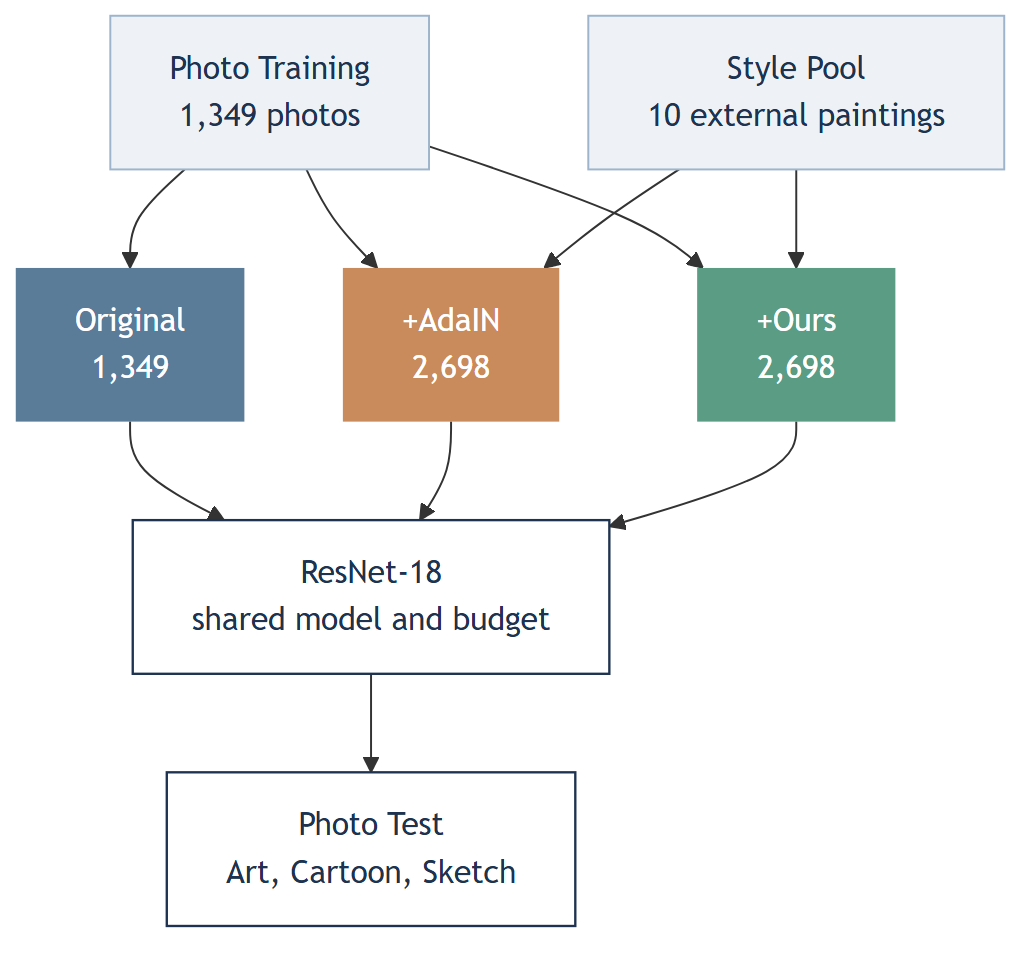
\includegraphics[width=\columnwidth]{figures/framework.png}%
  }{%
    \fbox{\parbox[c][2.2cm][c]{\dimexpr\columnwidth-2\fboxsep-2\fboxrule\relax}{\centering Placeholder: overall framework figure (planned).}}%
  }%
}
\caption{Overall framework. Photo Training images feed three training sets: originals only, originals plus AdaIN stylizations, and originals plus structure-preserving stylizations. Both stylized sets draw their style references from one frozen pool of external paintings. A single ResNet-18 training and evaluation protocol is applied to all three groups.}
\label{fig:framework}
\end{figure}

Stylized training images are produced \textit{offline}. Member 2's AdaIN generator and member 3's structure-preserving generator each write images to disk together with a manifest that records the content image, the style image, the style strength $\alpha$, and, for the structure-preserving variant, the structure parameter $\beta$. Training then reads from these fixed manifests, so the three groups go through an identical data-loading path. Nothing about the stylization is recomputed or resampled during classifier training, which keeps the classifier-side training code common to all groups.

Table~\ref{tab:groups} defines the three groups. The comparison Original vs.\ +AdaIN isolates the value of added style diversity (experiment 2), and +AdaIN vs.\ +Ours isolates the value of structure preservation (experiment 3), as detailed in Section~\ref{sec:exp_design}.

\begin{table}[t]
\caption{The three training groups. All groups use the same splits, model, and evaluation.}
\label{tab:groups}
\centering
\small
\setlength{\tabcolsep}{4pt}
\begin{tabular}{@{}lrr@{}}
\toprule
Group & Training images & Composition \\
\midrule
Original & 1{,}349 & Photo Training only \\
+AdaIN   & 2{,}698 & $+ 1{,}349$ AdaIN \\
+Ours    & 2{,}698 & $+ 1{,}349$ structure-preserving \\
\bottomrule
\end{tabular}
\end{table}

%==================================================

% Member 4 - Section 3.3 ResNet-18 Baseline
\subsection{ResNet-18 Baseline}
\label{sec:resnet_baseline}

We use ResNet-18~\cite{he2016resnet} as the classifier for all groups. It is the standard backbone for PACS-style domain generalization studies, and its moderate size fits our single-GPU compute budget while leaving room for multi-seed replication.

The network is initialized with ImageNet-pretrained weights, and the final fully connected layer is replaced with a seven-way classifier head. All layers are fine-tuned jointly. Pretraining matters in our setting: Photo Training has only 1{,}349 images, and training the same architecture from scratch on this amount of data yields a weak baseline that would compress the dynamic range of all comparisons.

\textit{Input transforms.} Training uses RandomResizedCrop to $224\times224$ with scale $(0.7, 1.0)$ and a horizontal flip, followed by ImageNet normalization. Evaluation resizes the shorter side to 256, center-crops to $224\times224$, and applies the same normalization. We deliberately exclude photometric augmentation such as color jitter and grayscale: those transformations change style-related statistics, which is exactly the variable under study, so adding them to all groups would confound the comparison. Geometric augmentation only is applied, identically in all groups.

\textit{Optimization.} All groups are trained with SGD (momentum 0.9, weight decay $5\times10^{-4}$, label smoothing 0.1~\cite{szegedy2016rethinking}), initial learning rate 0.01, batch size 64, and a cosine schedule~\cite{loshchilov2017sgdr} over a fixed step budget of 660 optimizer steps (Section~\ref{sec:exp_design}). We report the \textit{final} checkpoint of that budget, with no checkpoint selection on any validation split: we measured that selecting on Photo Validation accuracy inflates the seed-to-seed spread of cross-domain accuracy, and the measurement is reported in Section~\ref{sec:training_prep}. Target-domain test sets never influence training, checkpoint selection, or any hyperparameter choice.

% TODO (Member 2): \subsection{AdaIN Style Augmentation}
% TODO (Member 3): \subsection{Structure-Preserving Style Augmentation}

%==================================================

% Member 4 - Section 3.6 Evaluation Metrics
\subsection{Evaluation Metrics}
\label{sec:evaluation_metrics}

\textit{Classification accuracy.} We report top-1 accuracy on Photo Test (in-domain) and on each of Art Painting, Cartoon, and Sketch (cross-domain). The primary metric is the unweighted average of the three cross-domain accuracies. Every configuration is run with three training seeds; we report mean and standard deviation over seeds, and per-domain breakdowns are included so that effects which appear in only one domain are visible.

\textit{Structure preservation.} To characterize the generated data rather than the classifier, we compare each stylized image with its content image using two measures. The first is LPIPS~\cite{zhang2018lpips}, a perceptual distance between the two images; larger values mean the stylization moved the image further from its content. The second is \textbf{EdgeScore}, an edge-consistency measure built from Canny edge maps~\cite{canny1986}. Writing $E_c$ and $E_s$ for the binary edge maps of the content and the stylized image, we report

\[
\text{EdgeScore} = \frac{2PR}{P+R}, \quad
P = \frac{|E_c \cap E_s|}{|E_s|}, \quad
R = \frac{|E_c \cap E_s|}{|E_c|},
\]

which is the F1-style overlap of the two edge maps: it is 1 when the stylized image reproduces all of the content's contours and falls as the stylization erases them. Note that this is an \textit{overlap}, not a difference: it is the harmonic mean of the fraction of stylized edges that coincide with a content edge (precision) and the fraction of content edges that survive in the stylized image (recall). A plain edge difference would score a stylization that adds many spurious edges but keeps the content's contours as poorly as one that erases them, whereas EdgeScore rewards agreement in both directions. Canny thresholds are held fixed across all images so that scores are comparable. These metrics describe how much structure the generated data removes; they are analysis metrics and do not enter training or model selection.

%==================================================

% Member 4 - Section 3.7 Experimental Design and Fair Comparison
\subsection{Experimental Design and Fair Comparison}
\label{sec:exp_design}

\textit{Experiments.} Four experiments answer the four research questions in the Introduction. Experiment 1 trains the Original group and measures the Photo-versus-target gap. Experiment 2 compares Original against +AdaIN. Experiment 3 compares +AdaIN against +Ours with everything else held fixed. Experiment 4 sweeps the style strength $\alpha \in \{0.25, 0.5, 0.75, 1.0\}$ for both augmentation methods, tracing the relation between stylization strength, structure preservation, and cross-domain accuracy. A $\beta$ ablation for the structure-preserving method is planned alongside Experiment 4 (Section~5.3).

\textit{Fairness controls.} Because the compared methods differ only in their training images, the following quantities are fixed across groups:

\begin{itemize}
\item \textit{Same original data:} all groups train on the identical 1{,}349 Photo Training images from Table~\ref{tab:splits}.
\item \textit{Same style pool:} both augmented groups draw style references from one frozen pool of 10 style images, fixed with a content-hash manifest before any training run. The pool holds external paintings that are not part of PACS, and the checker verifies this mechanically (the ``No test-set leakage'' item below).
\item \textit{Same augmentation count:} each augmented group adds exactly one stylized image per original training image (1{,}349 added images).
\item \textit{Same content--style pairing:} the style image paired with each content image is drawn once with a fixed seed and reused by both generators, so the only difference between the two augmented datasets is the stylization algorithm itself.
\item \textit{Same transform pipeline and classifier:} one training script, one transform definition, one ResNet-18 configuration for all groups.
\item \textit{Same optimization budget:} all groups receive the same number of optimizer steps, $S = 660$, computed as 30 passes over the Original training set at batch size 64 ($30 \times 22$). Groups with larger training sets accordingly run fewer passes over their data. Validation is evaluated at the same step cadence for every group.
\item \textit{Same evaluation and seeds:} all groups use the test lists of Table~\ref{tab:splits} and are run with seeds $\{0, 1, 2\}$.
\item \textit{No checkpoint selection:} the reported model is the final checkpoint of the fixed step budget, for every group and every seed. This removes a selection step that we measured to be harmful (Section~\ref{sec:resnet_baseline}).
\item \textit{No test-set leakage:} the style pool is built from external paintings and contains no PACS image. Because Art Painting, Cartoon, and Sketch are the evaluation domains, a style reference drawn from any of them would place the test appearance into the training set. The checker compares the content hash of every style image against the whole local PACS copy and rejects the run if any style image is a PACS image.
\item \textit{Fairness verification.} A checker script validates these constraints mechanically before training: it confirms that the augmented manifests contain the same original images, the same style pool hash, the same augmentation count, that the content--style pairing is identical in both manifests, that no style image is a PACS image, and that the training configuration fingerprint is identical across groups. The configuration fingerprint is recomputed from the full training configuration recorded in each run summary, so a run whose hyper-parameters differ is rejected. A run that fails any check is excluded from results.
\end{itemize}

\textit{Reporting.} Table~\ref{tab:results} shows the result table format used throughout. Entries are mean$\pm$standard deviation over three seeds. Differences between groups are reported per seed, so that a gain which depends on one favorable seed is visible rather than hidden in the average.

\begin{table}[t]
\caption{Result table. Entries are mean$\pm$standard deviation over three training seeds. The Original row is complete (experiment 1); the two augmented rows are pending delivery of the stylization manifests.}
\label{tab:results}
\centering
\scriptsize
\setlength{\tabcolsep}{2.5pt}
\begin{tabular}{@{}lccccc@{}}
\toprule
Training method & Photo & Art & Cartoon & Sketch & Avg \\
\midrule
Original & $99.0\pm0.3$ & $63.2\pm3.7$ & $25.1\pm1.8$ & $31.5\pm4.2$ & $39.9\pm2.7$ \\
+AdaIN   & -- & -- & -- & -- & -- \\
+Ours    & -- & -- & -- & -- & -- \\
\bottomrule
\end{tabular}
\end{table}

Experiment 1 is complete. The Original group reaches $99.0\%$ on Photo Test but only $39.9\%$ averaged over the three unseen domains, so the domain gap is both large and unambiguous. The gap is not uniform: Art Painting, whose appearance is closest to photography, is recognized at $63.2\%$, whereas Cartoon and Sketch, which discard most photographic cues, fall to $25.1\%$ and $31.5\%$. This ordering is the one we would expect from a classifier that relies mainly on photographic texture, and it identifies Cartoon and Sketch as the domains where style augmentation has the most room to help.

\begin{figure}[t]
\centering
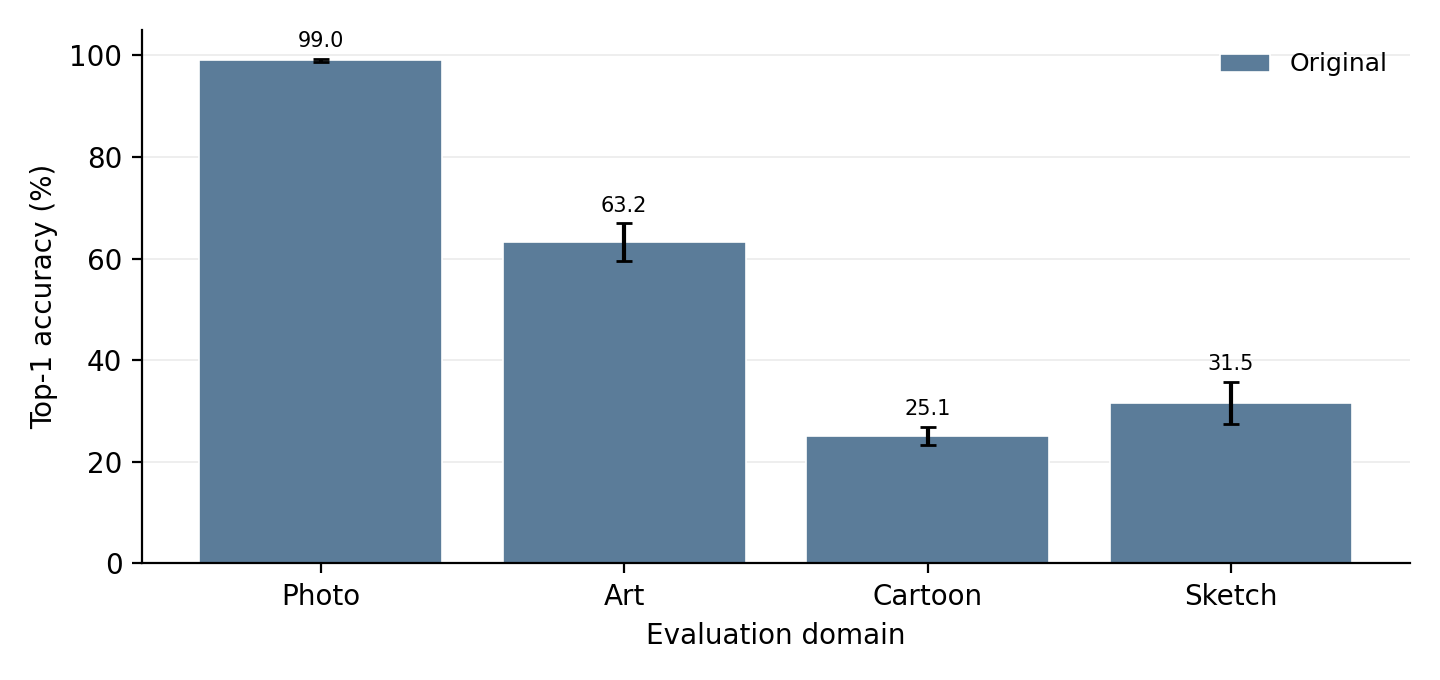
\includegraphics[width=\columnwidth]{figures/results_baseline.png}
\caption{Experiment 1: accuracy of the Original group on the in-domain Photo test set and on the three unseen target domains. Bars are means over three seeds; whiskers are standard deviations.}
\label{fig:results_baseline}
\end{figure}

%==================================================

%==================================================

% Member 4 - Section 5.2 Experiment Completion Plan
\subsection{Experiment Completion Plan}
\label{sec:completion_plan}

The unified training and evaluation code is complete and validated on the local PACS copy, so the remaining experiment work is primarily GPU time. The plan below assumes the two generators are delivered by their owners in week 1; the frozen style pool they will use is already in place (Section~\ref{sec:exp_design}).

\begin{itemize}
\item \textit{Week 1: Experiment 1 and baseline replication.} \textit{Done.} The Original group has been run with seeds $\{0,1,2\}$ on the fixed 660-step budget, giving $99.0\pm0.3\%$ in-domain and $39.9\pm2.7\%$ cross-domain. The step budget was fixed before these runs (30 nominal passes over the training set). A diagnostic run to 1{,}320 steps, recorded but not used for tuning, shows that cross-domain accuracy fluctuates within a narrow band from the first evaluation onwards rather than improving systematically with more steps; the budget was therefore kept at 660 steps for all groups and every group reports its final checkpoint (Section~\ref{sec:resnet_baseline}). The remaining work in this week is to fix the checkpoint-selection policy, which we have done (Section~\ref{sec:resnet_baseline}), and to confirm the final protocol with the group.
\item \textit{Week 2: Experiments 2 and 3.} Generate the two augmented datasets from the frozen style pool and run +AdaIN and +Ours with the same three seeds. Run the fairness checker on both augmented manifests before training.
\item \textit{Week 3: Experiment 4 and ablation.} Sweep $\alpha \in \{0.25, 0.5, 0.75, 1.0\}$ for both methods on one seed, plus the $\beta$ sweep for the structure-preserving method; compute LPIPS and EdgeScore (Section~\ref{sec:evaluation_metrics}) on all generated datasets.
\item \textit{Week 4: Replication and analysis.} Re-run the best configurations on the remaining seeds, assemble per-domain and per-class tables, and identify where structure preservation helps or fails.
\end{itemize}

Compute budget: one training run takes roughly 10 minutes on the project GPU (RTX 4070 Laptop, 8\,GB), so the full plan above totals approximately 15--20 GPU-hours including sweeps and reruns, which fits the available hardware within the schedule.

% TODO (Member 5): 5.1, 5.4, 5.5

%==================================================

%==================================================


%==================================================
\begin{thebibliography}{00}

\bibitem{zhou2023dgsurvey}
K.~Zhou, Z.~Liu, Y.~Qiao, T.~Xiang, and C.~C.~Loy,
``Domain generalization: A survey,''
\textit{IEEE Trans. Pattern Anal. Mach. Intell.}, vol.~45, no.~4, pp.~4396--4415, 2023.

\bibitem{zhou2021mixstyle}
K.~Zhou, Y.~Yang, Y.~Qiao, and T.~Xiang,
``Domain generalization with MixStyle,''
in \textit{Proc. Int. Conf. Learning Representations (ICLR)}, 2021.

\bibitem{huang2017adain}
X.~Huang and S.~Belongie,
``Arbitrary style transfer in real-time with adaptive instance normalization,''
in \textit{Proc. Int. Conf. Computer Vision (ICCV)}, 2017.

\bibitem{li2017dg}
D.~Li, Y.~Yang, Y.-Z.~Song, and T.~Hospedales,
``Deeper, broader and artier domain generalization,''
in \textit{Proc. Int. Conf. Computer Vision (ICCV)}, 2017.

\bibitem{zhou2020dassl}
K.~Zhou, ``Dassl: Domain adaptation and generalization library,''
\url{https://github.com/KaiyangZhou/Dassl.pytorch}, accessed 2026.

\bibitem{he2016resnet}
K.~He, X.~Zhang, S.~Ren, and J.~Sun,
``Deep residual learning for image recognition,''
in \textit{Proc. IEEE Conf. Computer Vision and Pattern Recognition (CVPR)}, pp.~770--778, 2016.

\bibitem{zhang2018lpips}
R.~Zhang, P.~Isola, A.~A.~Efros, E.~Shechtman, and O.~Wang,
``The unreasonable effectiveness of deep features as a perceptual metric,''
in \textit{Proc. IEEE Conf. Computer Vision and Pattern Recognition (CVPR)}, 2018.

\bibitem{canny1986}
J.~Canny,
``A computational approach to edge detection,''
\textit{IEEE Trans. Pattern Anal. Mach. Intell.}, vol.~8, no.~6, pp.~679--698, 1986.

\bibitem{szegedy2016rethinking}
C.~Szegedy, V.~Vanhoucke, S.~Ioffe, J.~Shlens, and Z.~Wojna,
``Rethinking the Inception architecture for computer vision,''
in \textit{Proc. IEEE Conf. Computer Vision and Pattern Recognition (CVPR)}, 2016.

\bibitem{loshchilov2017sgdr}
I.~Loshchilov and F.~Hutter,
``{SGDR}: Stochastic gradient descent with warm restarts,''
in \textit{Proc. Int. Conf. Learning Representations (ICLR)}, 2017.

\end{thebibliography}

\end{document}
